\documentclass[12pt]{report}

\setlength{\parskip}{1em}
\usepackage{indentfirst}

\usepackage{fancyhdr}
\usepackage{float}
\usepackage[letterpaper]{geometry}
\usepackage{graphicx}
\usepackage{lastpage}

\pagestyle{fancy}
\fancyhf{}

\fancyhead[RE,RO]{Distributed Automotive Sensor/Actuator Network}
\fancyfoot[LE,LO]{
  \jobname{.tex}
}

\fancyfoot[CE,CO]{\thepage\ of \pageref{LastPage}}
\fancyfoot[RE,RO]{
    \today
}

\geometry{verbose,tmargin=1in,bmargin=1in,lmargin=1in,rmargin=1in}

\renewcommand*\thesection{\arabic{section}.}
\renewcommand*\thesubsection{\arabic{section}.\arabic{subsection}.}

\begin{document}

\title{Distributed Automotive Sensor/Actuator Network}
\author{
	\hline
	ECE 4600 Progress Report\\
	for the period from
	\\2009-09-01 to 2009-12-31\\
	\hline
	\\ \\
	\textbf{Faculty Advisor}\\
	Dr. Witold Kinsner, Ph.D., P.Eng., University of Manitoba\\
	\\
	\textbf{Submitted by}\\
	John Hughes\\
	Michael Jean
	\\ \\
	\textbf{Submitted on}
	\vspace{-1em}
}
\maketitle

\section{Summary}

The goal of this project is to deliver four control modules for the UMSAE 2010 Formula racing vehicle. The four modules are:
\begin{itemize}
 \item an Engine and Transmission Control Module;
 \item a Braking Control Module;
 \item a Wireless Telemetry Module;
 \item and Driver Interface Module.
\end{itemize}
The project is progressing, however significant delays in the manufacturing of printed circuit boards and the acquisition of sponsorship funding to purchase parts has put the project two months behind schedule when compared to predictions made in the project proposal document. In hindsight, the initial timeline proposed did not consider possible delays and was far too optimistic. The funding and supplier issues have been resolved and a revised schedule still allows for delivery of all four modules on time. 

\pagebreak

\section{Background}

As mentioned previously, the goal of the project is to deliver four control modules for the UMSAE 2010 Formula racing vehicle. Each module consists of a printed circuit board containing all the necessary circuitry, wiring harnesses, a weater-proof and shock-proof enclosure to house the physical components, wiring to connect all of the modules to each other and to the various sensors and actuators throughout the vehicle, and software necessary to perform the tasks of each controller.

The \emph{Engine and Transmission Control Module} allows the driver to change gears by paddles, eliminating the need to manually clutch. This reduces driver effort required and increases vehicle performance. The module also controls the length of the intake runners, implementing a 2-stage variable intake plenum, which improves power output from engine under certain operating conditions.

The \emph{Braking Control Module} allows the driver to adjust the brake bias, that is, the distribution of braking force between the front and rear wheels. This improves driver control over the vehicle and overall driver safety. It also improves performance of the vehicle and eliminates the need for imprecise and impractical manual tuning of the brake bias.

The \emph{Wireless Telemetry Module} relays information from the various vehicle sensors back to the pit crew over a wireless link. The module incorporates a third-party XBee Pro wireless modem to accomplish the wireless link. Specialized software running on laptops held by the pit crew interpret the information in real-time. This software is third-party and has already been provided to us.

The \emph{Driver Interface Module} is contained within the steering wheel of the vehicle and contains an LCD screen with several knobs and buttons used to adjust settings for the various control modules. The LCD provides feedback to the driver regarding the current state of the vehicle, including wheel speed, engine RPM, fuel level, et cetera. 

The modules are interconnected with an \emph{Controller Area Network} (CAN) that enables quick, error-resiliant communications with only two wires.

\pagebreak

\section{Project Status}

  The project is approximately two months behind schedule. The Project is within budget constraints. All components have been ordered and all 4 PCBs have been manufactured and are in our hands, waiting to be populated.

  \subsection{Progress}

  Several of the milestones have been pushed forward by at least two months. This is due to four major factors:
  \begin{enumerate}
  \item Over-optimistic initial planning due to lack of project management experience of this sort by both team members;
  \item Under-estimation of the amount of effort that other coursework required;
  \item Significant delays (over two months) in the manufacturing of the printed circuit boards due to manufacturer demand; and
  \item Critical delays in funding promised from UMSAE sponsors, resulting in the inability to acquire parts and manufacturing facilities in a timely manner.
  \end{enumerate}

  Table \ref{table:milestones} below lists the Project Milestones with their original target date, current status, and new target date.

  \begin{table}[H]
    \caption{Project milestones.}
    \label{table:milestones}
    \centering
    \begin{tabular}{|l|c|c|r|}
      \hline
      Task & Original Target & Status & New Target\\
      \hline
      Project Proposal Due & 2009/10/09 & Completed & N/A \\
      PCB Design Complete & 2009/10/15 & Completed & N/A  \\
      PCBs Manufactured & 2009/10/30 & Completed & N/A \\
      PCBs Populated and Tested & 2009/11/04 & Revised & 2010/01/12 \\
      Pneumatic System Modelled & 2009/11/15 & Revised & 2010/01/15 \\
      CAN Tester & 2009/11/30 & Revised & 2010/01/21 \\
      Software Written & 2009/12/02 & Revised & 2010/02/05 \\
      \hline
    \end{tabular}
  \end{table}

  Each team member has been working for at least twenty hours per week on the project, on average.

  Hardware design of all four modules has been completed by John Hughes. He has submitted his designs to the PCB manufacturer and has received the completed circuit boards back. Two industry contacts have been contacted with regards to assistance in populating the PCBs, which could dramatically reduce the amount of time required for this stage of the project. He has also managed the required material logistics for each module and submitted orders to Digikey. He has begun working on the wireless telemetry software, in collaboration with a computer science undergraduate. John has also initiated the pneumatic system modelling, which will hopefully proceed in collaboration with the mechanical engineering student Jose M Ricon Ruiz.

  Software design of all four modules has been completed by Michael Jean. He has acquired a development board to begin early hardware tests, and written a suite of test software for the newly manufactured PCBs. He has written drivers for several of the major microcontroller subsystems such as the CAN and SPI interfaces. When the modules are fully populated, he will begin implementing the various embedded software controllers for each module. He is currently finishing the implementation of the CAN testing device.

  Early designs called for an electromechanical motor based actuation of the clutch and gear levers. Further testing proved this infeasable, and a pneumatic design was instead proposed. This system is currently being modelled in Simulink. A controller for the shift system will then be designed from this model.

  \subsection{Future Plans}

  Great efforts have been expended on behalf of both team members. John Hughes has currently completed a large share of his designated tasks for the project. As he is the principle hardware designer, and Michael Jean is the principle software designer, it is only natural that the hardware tasks would be completed before all of the software tasks. It is expected that the work load on John Hughes will be lighter during the last half of the project, while it will be heavier for Michael Jean.

  The next steps are:
  \begin{enumerate}
  \item Populate printed circuit boards;
  \item Complete and validate transmission control system; and
  \item Implement embedded software on all four modules.
  \end{enumerate}

  \pagebreak

  \section{Conclusions}

  The project scope has not changed since the initial project proposal, however an over-optomistic timeline and heavy courseload has caused some trouble for the group, namely the project time-line has shifted forward about two months. The project will still be completed under budget and within the time limits allowed. 

  \pagebreak

  \section*{Appendix 1 - Parts Ordered/Received}

  Table \ref{table:parts_ordered} lists the parts currently on order from digikey that are required for the project. Certain parts are on backorder from Digikey, or must be sourced from a different supplier. These are not listed.\\

  The four custom printed circuit boards have been ordered and received.

  \begin{table}[H]
    \caption{Parts ordered.}
    \label{table:parts_ordered}
    \centering
    \begin{small}
    \begin{tabular}[c]{|l|l|l|l|l|}
    \hline
    Qty&Part Number&Description&Unit&Total\\
    \hline
    45&PCC1870CT&CAP .1UF 16V CERAMIC X7R 1206&0.26&\$11.79\\
    20&311-1177-1&CAP 33000PF 50V CERAMIC X7R 1206&0.12&\$2.46\\
    5&PCE4008CT&CAP 47UF 25V ELECT FC SMD&0.5&\$2.49\\
    10&311-1151-1&CAP CERAMIC 15PF 50V NP0 1206&0.14&\$1.36\\
    20&311-1154-1&CAP CERAMIC 22PF 50V NP0 1206&0.14&\$2.72\\
    10&399-3694-1&CAPACITOR TANT 3.3UF 10V 10\% SMD&0.19&\$1.88\\
    4&535-9071-1&CRYSTAL 16.000MHZ 18PF FUND SMD&0.63&\$2.50\\
    3&535-9034&CRYSTAL 32.768KHZ 12.5PF CYL&0.28&\$0.84\\
    1&296-3051-5&IC 8 BIT 3US DAC S/O 8-MSOP&3.49&\$3.49\\
    1&296-8441-5&IC BUFF/DVR HEX NON-INV 14SOICN&0.59&\$0.59\\
    4&LT1129CST-5&IC LDO REG W/SD 5V SOT223-3&5.1&\$20.40\\
    4&AT90CAN128&IC MCU AVR FLASH 128K 64-TQFP&15.35&\$61.40\\
    1&620-1140-1&IC MOTOR DRIVER PWM FULL 24SOIC&4.84&\$4.84\\
    4&LTC1232CS8&IC MPU SUPERVISORY CIRCUIT 8SOIC&4.31&\$17.24\\
    4&MCP2551-I/SN&IC TRANSCEIVER CAN HI-SPD 8-SOIC&1.27&\$5.08\\
    10&P11518CT&LED RED (UP) W/LENS 1206&0.42&\$4.24\\
    10&P595CT&LED YEL/GRN CLEAR DOME-LENS SMD&0.59&\$5.86\\
    10&RHM100KFCT&RES 100K OHM 1/4W 1\% 1206 SMD&0.05&\$0.54\\
    10&P120ECT&RES 120 OHM 1/4W 5\% 1206 SMD&0.11&\$1.06\\
    30&P499FCT&RES 499 OHM 1/4W 1\% 1206 SMD&0.13&\$3.99\\
    4&P13597SCT&SWITCH LT TOUCH 6X3.5 160GF SMD&0.65&\$2.60\\
    \hline
    &&&&\\
    Total&&&&\$157.37\\
    &&&&\\
    \hline
    \end{tabular}
    \end{small}
  \end{table}

  \pagebreak

  \section*{Appendix 2 - Updated Gantt Chart}

  Figure \ref{fig:gantt} below is the project's Gantt chart updated to reflect the current progress in each of our tasks. Filled bars show completion of a task.

  \begin{figure}[H]
  \centering{}
    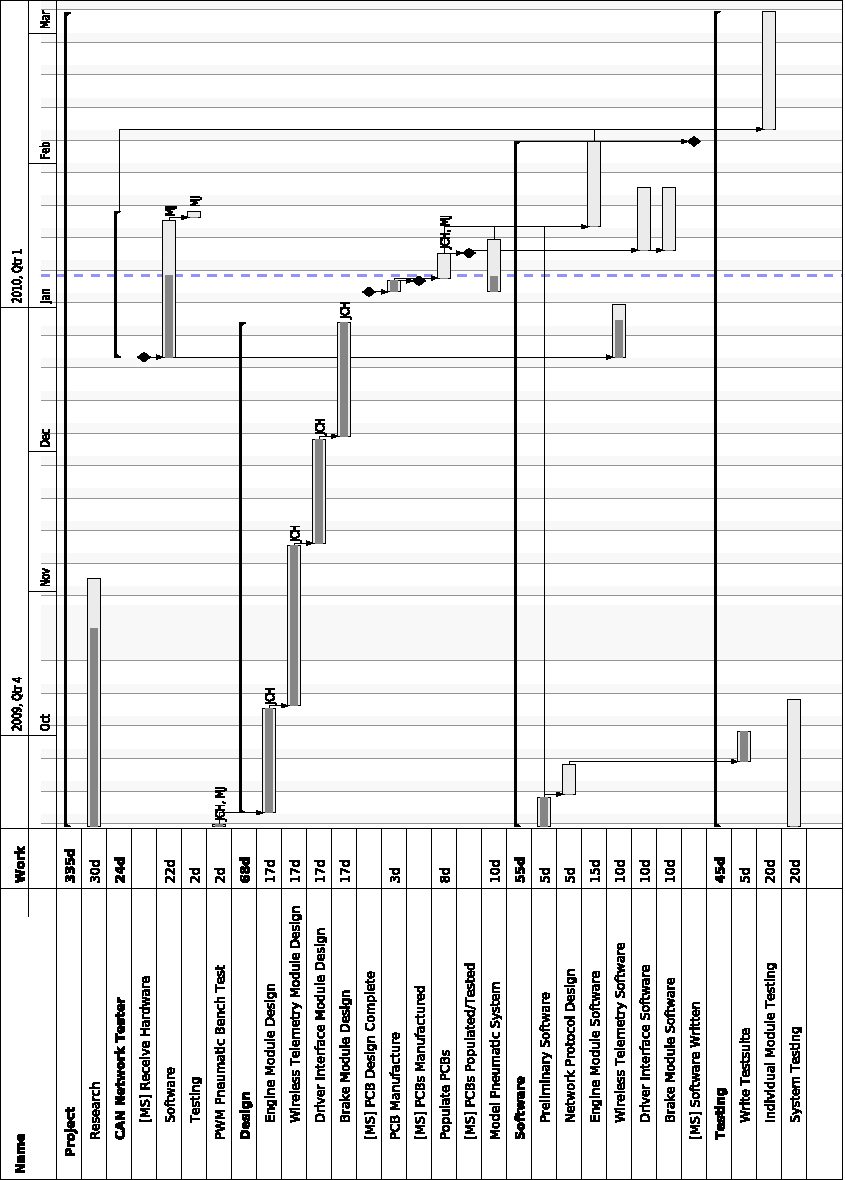
\includegraphics[width=0.75\columnwidth]{gantt_chart.pdf}

  
  \begin{flushleft}
  \caption{Updated Gantt chart.}
  \end{flushleft}

  \label{fig:gantt}
  \end{figure}

  \pagebreak

  \section*{Appendix 3 - Budget}

  The items that could have potentially costed the most have been the custom printed circuit boards. The cost of manufacturing these has however been covered by the manufacturer. The current cost of components to populate the boards has actually been lower than initially expected. Where possible, parts already in the posession of UMSAE have been used, such as the XBee modem modules, which were purchased last year and never used. Any costs exceeding the \$200 capstone budget will be covered by the UMSAE sponsorship budget, however the timely nature of this cannot be guaranteed. Table \ref{tab:budget} below outlines the current parts aquisition expenditures.

    \begin{table}[H]
      \begin{centering}
	\caption{Current budget useage}\label{tab:budget}
	\begin{tabular}{|l|r|}
	  \hline 
	  \textbf{Item} & \textbf{Cost}\tabularnewline
	  \hline
	  \hline 
	  Braking Module PCB & \$113.16\tabularnewline
	  \hline 
	  Telemetry Module PCB & \$127.65\tabularnewline
	  \hline 
	  Interface Module PCB & \$173.87\tabularnewline
	  \hline 
	  Engine Module PCB & \$113.16\tabularnewline
	  \hline 
	  PCB Shipping & \$28.00\tabularnewline
	  \hline
	  \hline 
	  \textbf{Total cost of PCBs} & \textbf{\$555.84}\tabularnewline
	  \hline
	  \hline 
	  Digikey parts currently ordered & \$157.37\tabularnewline
	  \hline 
	  Required parts on backorder/to be sourced & \$62.05\tabularnewline
	  \hline
	  \hline 
	  \textbf{Total cost of parts} & \textbf{\$219.42}\tabularnewline
	  \hline
	\end{tabular}
	\par
      \end{centering}
    \end{table}

\pagebreak

\end{document}